\documentclass[11pt]{article}
\usepackage[margin = 1in]{geometry}
\usepackage{amsmath}
\usepackage{amssymb}
\usepackage{amsthm}
\usepackage{graphicx}
\usepackage{subfig}
\usepackage{enumitem}
\usepackage{url}
\usepackage[parfill]{parskip}
\usepackage{listings}
\newcommand{\cvector}[2]{\begin{pmatrix} #1 \\ #2 \end{pmatrix}}
\newcommand{\smatrix}[4]{\begin{pmatrix} #1 & #2 \\ #3 & #4 \end{pmatrix}}
\newcommand{\skipline}{\vspace{\baselineskip}}
\newenvironment{problem}[1]{\textbf{Problem #1: }}{\newpage}

\usepackage[utf8]{inputenc}
\usepackage{xcolor}

\definecolor{codegreen}{rgb}{0,0.6,0}
\definecolor{codegray}{rgb}{0.5,0.5,0.5}
\definecolor{codepurple}{rgb}{0.58,0,0.82}
\definecolor{backcolour}{rgb}{0.95,0.95,0.92}

\lstdefinestyle{mystyle}{
	backgroundcolor=\color{backcolour},   
	commentstyle=\color{codegreen},
	keywordstyle=\color{magenta},
	numberstyle=\tiny\color{codegray},
	stringstyle=\color{codepurple},
	basicstyle=\ttfamily\footnotesize,
	breakatwhitespace=false,         
	breaklines=true,                 
	captionpos=b,                    
	keepspaces=true,                 
	numbers=left,                    
	numbersep=5pt,                  
	showspaces=false,                
	showstringspaces=false,
	showtabs=false,                  
	tabsize=2
}

\lstset{style=mystyle}
\begin{document}
	
	\begin{center}
		\textbf{Assignment 3} \\
		\textbf{Computer Vision} \\
		\textbf{CS 559} \\
		\textbf{Stephen Giang RedID: 823184070} \\
		\skipline \skipline
	\end{center}

	\begin{problem}{1}
		\begin{enumerate}[label = (\alph*)]
			\item Let $f(x,y)$ be an image.  Let $h(x,y)$ be the image obtained by applying a 3 by 3 spatial low pass mask (averaging filter) to $f(x,y)$.  Similarly let $g(x,y)$ be the image obtained by applying a 3 by 3 spatial high pass mask to $f(x,y)$.  Prove that
			\[g(x,y) = f(x,y) - h(x,y)\]
			\begin{proof}
				We can write $h(x,y)$ as the following as it is the spatial low pass mask:
				\begin{align*}
					h(x,y) &= \frac{1}{9} \bigg( f(x-1,y-1) + f(x,y-1) + f(x+1,y-1) + f(x-1,y)  \\
					&+ f(x,y) + f(x+1,y) + f(x-1,y + 1) + f(x,y + 1) + f(x+1,y + 1) \bigg)
				\end{align*}
				Notice the high pass filter for $g(x,y)$:
				\begin{align*}
					U = sE - \frac{s}{k}A = s\begin{pmatrix}
						0 & 0 & 0 \\ 0 & 1 & 0 \\ 0 & 0 & 0
					\end{pmatrix} - \frac{s}{k}\begin{pmatrix}
						1 & 1 & 1 \\ 1 & 1 & 1 \\ 1 & 1 & 1
					\end{pmatrix}
				\end{align*}
				We can see that if we let $s = 1$ and $k = 9$ and apply the filter to $f(x,y)$, we get:
				\begin{align*}
					g(x,y) = f(x,y) &- \frac{1}{9} \bigg( f(x-1,y-1) + f(x,y-1) + f(x+1,y-1) + f(x-1,y)  \\
					&+ f(x,y) + f(x+1,y) + f(x-1,y + 1) + f(x,y + 1) + f(x+1,y + 1) \bigg)
				\end{align*}
				Thus we get that
				\[g(x,y) = f(x,y) - h(x,y)\]
			\end{proof}
			\skipline
			\item Is the high pass mask separable? What is the implication of separability on computations?
			\\ \\
			We have the high pass mask in the form of:
			\[U = \frac{s}{k}\begin{pmatrix}
				-1 & -1 & -1 \\ -1 & k - 1 & -1 \\ -1 & -1 & -1
			\end{pmatrix}\]
			Because each row or each column are not scalar multiples of each other, we get that the high pass mask is not separable.  The implication of separability on computations is that it reduces the run-time complexity, thus saving a lot of computations.
		\end{enumerate}
	\end{problem}

	\begin{problem}{2}
		Find the output images if Sobel edge operators are applied to the following 8 by 8 input image.  Note that you will have three gradient images, one in x-direction, one in y-direction and one gradient magnitude. Ignore the border effects, and produce only 6 by 6 output images.
		\begin{verbatim}
			2   2   2   2   2   2   2   2
			2   2   2   2   2   2   2   7
			2   2   2   2   2   2   7   7
			2   2   2   2   2   7   7   7
			2   2   2   2   7   7   7   7
			2   2   2   7   7   7   7   7
			2   2   7   7   7   7   7   7 
			2   7   7   7   7   7   7   7	
		\end{verbatim}
		Notice the following Sobel masks:
		\[M_x = \begin{bmatrix}
			-1 & 0 & 1 \\ -2 & 0 & 2 \\ -1 & 0 & 1
		\end{bmatrix}, \qquad M_y = \begin{bmatrix}
			-1 & -2 & -1 \\ 0 & 0 & 0 \\ 1 & 2 & 1 
		\end{bmatrix}\]
		Notice the output images, $G_x$, $G_y$, $G_{mag}$:
		\[G_x = \begin{bmatrix}
			0 & 0 & 0 & 0 & 5 & 15 \\
			0 & 0 & 0 & 5 & 15 & 15 \\
			0 & 0 & 5 & 15 & 15 & 5 \\
			0 & 5 & 15 & 15 & 5 & 0 \\
			5 & 15 & 15 & 5 & 0 & 0 \\
			15 & 15 & 5 & 0 & 0 & 0
		\end{bmatrix} \qquad G_y = \begin{bmatrix}
			0 & 0 & 0 & 0 & 5 & 15 \\
			0 & 0 & 0 & 5 & 15 & 15 \\
			0 & 0 & 5 & 15 & 15 & 5 \\
			0 & 5 & 15 & 15 & 5 & 0 \\
			5 & 15 & 15 & 5 & 0 & 0 \\
			15 & 15 & 5 & 0 & 0 & 0
		\end{bmatrix} \]
		Notice to find the magnitude, we get $g_{mag}(x,y) = \sqrt{g_x(x,y)^2 + g_y(x,y)^2}$.  Thus because $g_x = g_y$, we have that $g_{mag} = \sqrt{2 (g_x)^2} = \sqrt{2}g_x$.  Thus we get the following:
		\[G_{mag} = \sqrt{2}\begin{bmatrix}
			0 & 0 & 0 & 0 & 5 & 15 \\
			0 & 0 & 0 & 5 & 15 & 15 \\
			0 & 0 & 5 & 15 & 15 & 5 \\
			0 & 5 & 15 & 15 & 5 & 0 \\
			5 & 15 & 15 & 5 & 0 & 0 \\
			15 & 15 & 5 & 0 & 0 & 0
		\end{bmatrix}\]
	\end{problem}

	\begin{problem}{3}
		The purpose of this programming assignment is to explore and then propose a good edge detection method for color images. Then identify the boundary of the object in the image that has a particular color. As an example consider the image below and find and mark the detected boundary of  the green pepper in a different color (say blue). Your program must work with other images. Now get another image of your choice and demonstrate your program. You can use Python/Matlab functions but you must understand how they work as this could be an exam/quiz question. 
		\begin{figure}[h!]
			\centering
			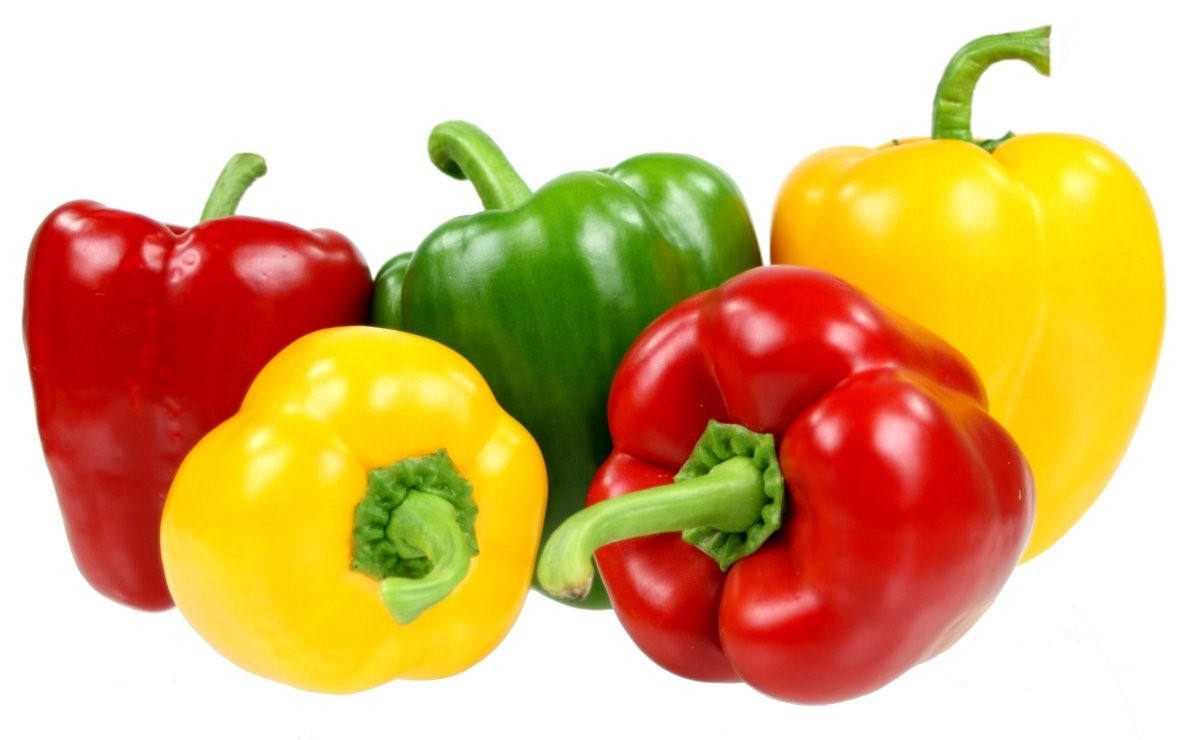
\includegraphics[width = 8cm]{Images/BellPepper3}
		\end{figure}
		\\
		Write a short report about any special feature of your program and  your findings, make comments and conclusions supported by images.
		\\ \\
		What I did with my code was I indexed through each pixel.  I then checked the left and right of each pixel.  If one side was green and the other side was not, then it would turn that pixel blue, and then I did the same vertically. Notice my images, with the following parameters.  For the Bell Pepper image, I set $redLim = 140, \,\,greenLim = 20,\,\, blueLim = 50$. For the Apple image, I set $redLim = 200,\,\, greenLim = 150,\,\, blueLim = 120$. 
		\begin{figure}[h!]
			\centering
			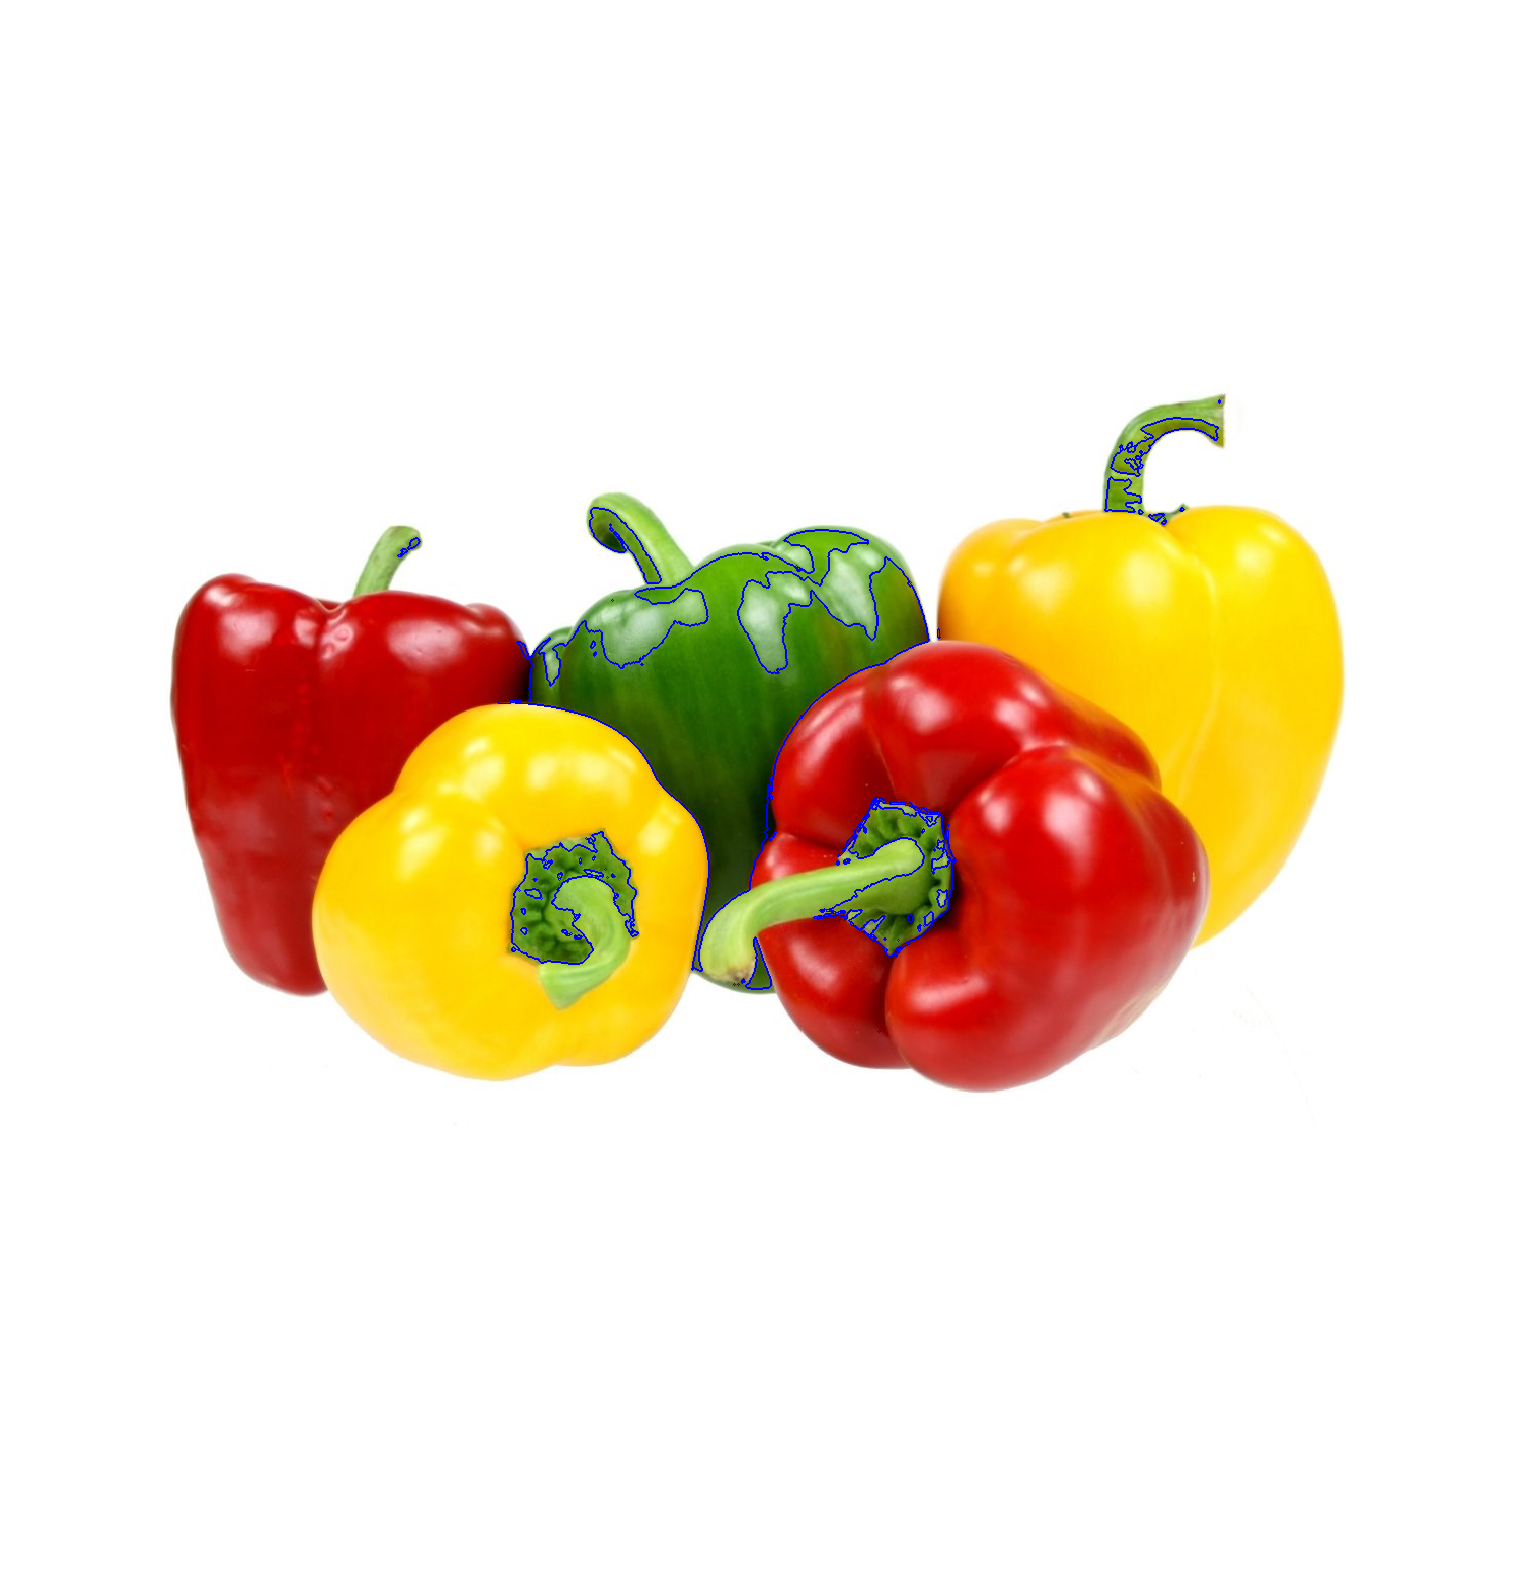
\includegraphics[width = 8cm]{Images/BellBlue}
			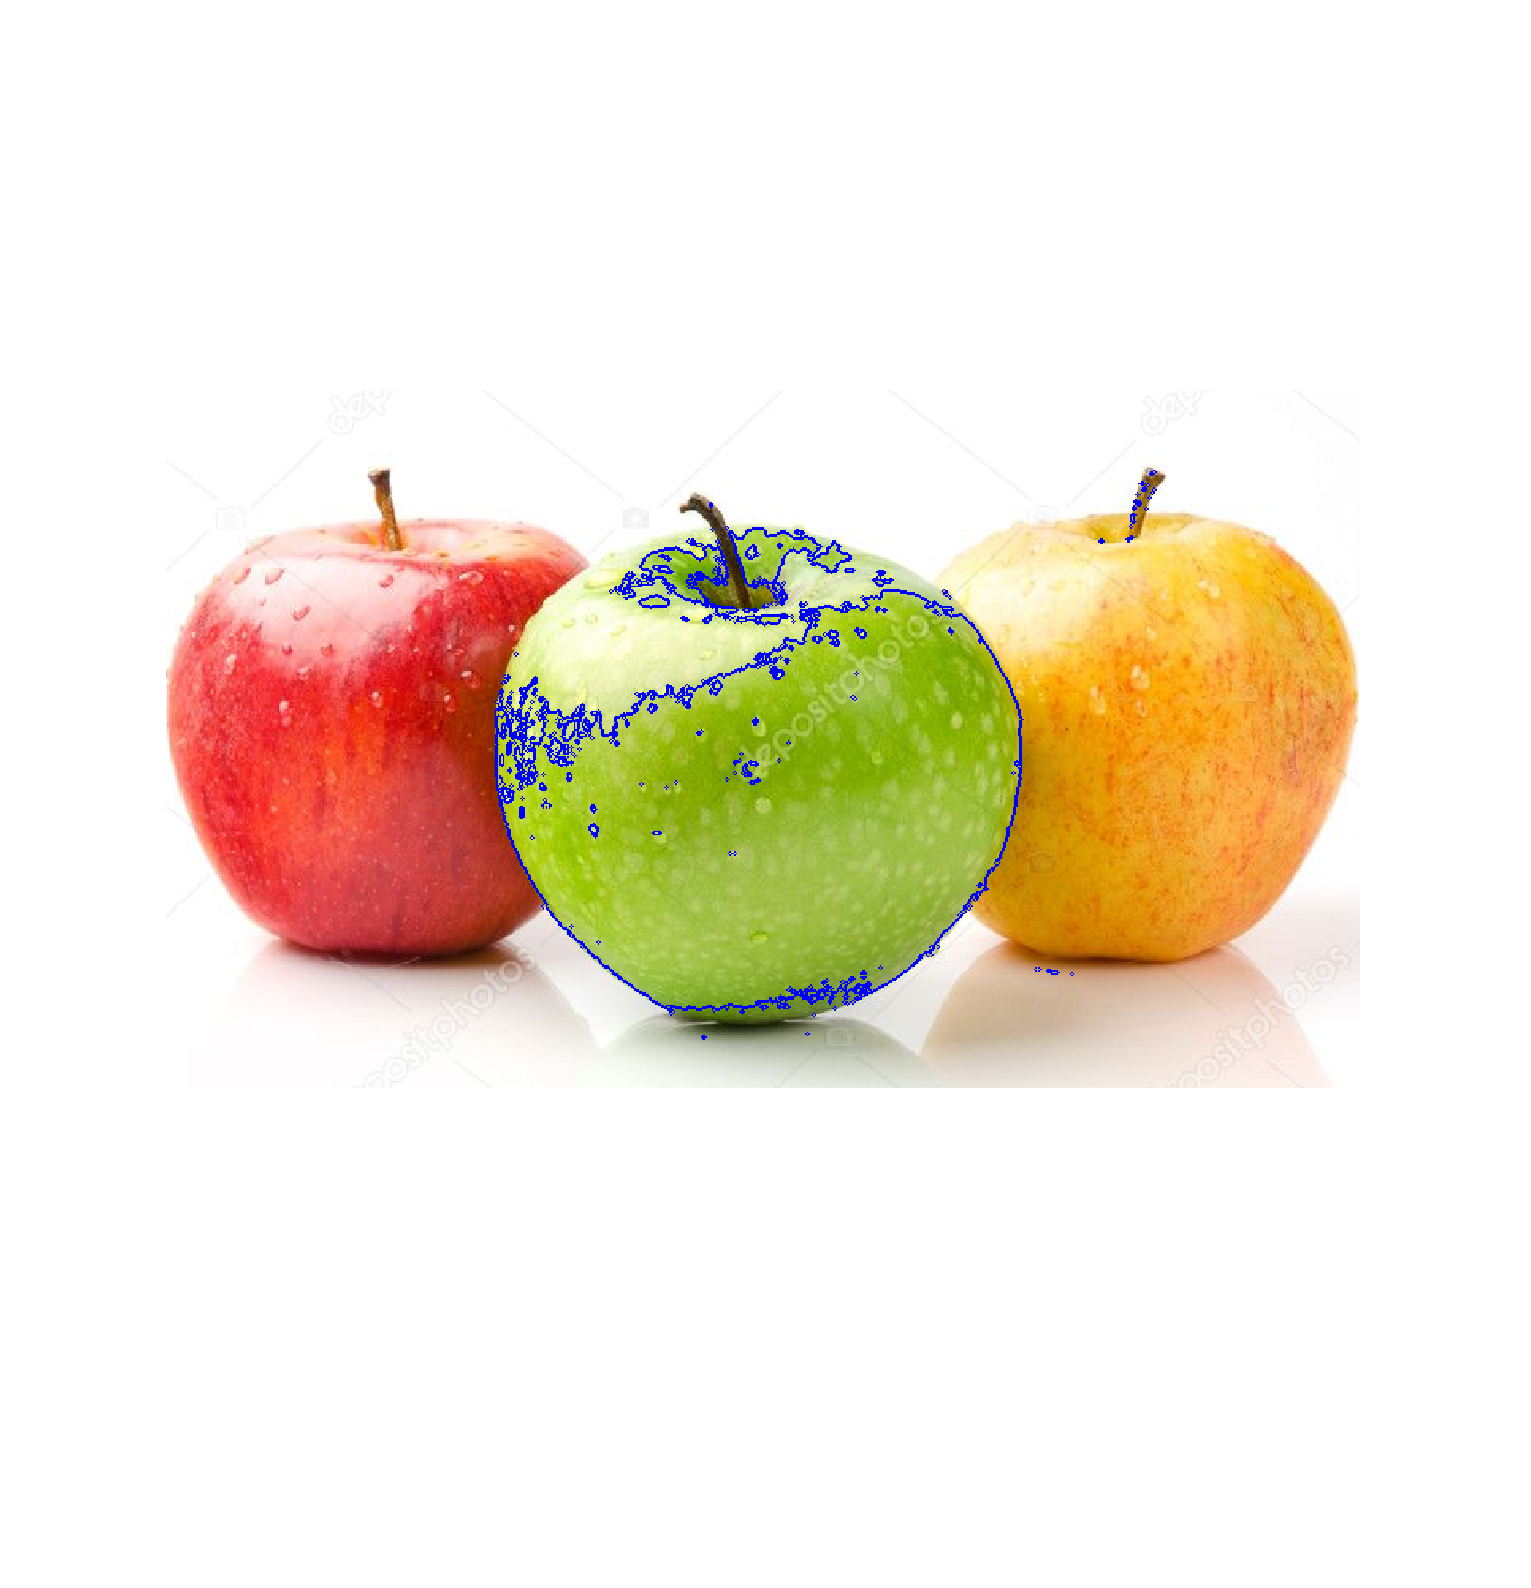
\includegraphics[width = 8cm]{Images/AppleBlue}
		\end{figure}
		\newpage
\begin{lstlisting}[language = Matlab]
function [] = colorEdgeDetect (fileName, redLim, greenLim, blueLim)

	input = imread(fileName);
	red = input(:,:,1);
	green = input(:,:,2);
	blue = input(:,:,3);
	output = input;
	
	% Horizontal Traversal
	for x = 2 : ( size(input, 1) - 2 )
		for y = 2 : ( size(input, 2) - 2 )
			greenLeft = red(x-1,y) < redLim && green(x-1,y) > greenLim && blue(x-1,y) < blueLim; 
			greenRight = red(x+1,y) < redLim && green(x+1,y) > greenLim && blue(x+1,y) < blueLim;
			if (greenLeft && ~greenRight) || (~greenLeft && greenRight)
				output(x,y,1) = 0;
				output(x,y,2) = 0;
				output(x,y,3) = 255;
			end      
		end
	end
	
	% Vertical Traversal
	for x = 2 : ( size(input, 1) - 2 )
		for y = 2 : ( size(input, 2) - 2 )
			greenLeft = red(x,y-1) < redLim && green(x,y-1) > greenLim && blue(x,y-1) < blueLim; 
			greenRight = red(x,y+1) < redLim && green(x,y+1) > greenLim && blue(x,y+1) < blueLim;
			if (greenLeft && ~greenRight) || (~greenLeft && greenRight)
				output(x,y,1) = 0;
				output(x,y,2) = 0;
				output(x,y,3) = 255;
			end      
		end
	end

	imshow(output)
end
\end{lstlisting}
		
	\end{problem}

	\begin{problem}{4}
		The purpose of this assignment is to detect the motion of a car (and its speed). Stay still and take two (or move) pictures of a moving car in your neighborhood (better put the camera on a stand so it remains still). Your task is to write a program that takes the two images as input and finds the physical (world) distance between two consecutive frames (from which the speed of the car can be determined, if you measure the time between two frames. Finding speed is not part of this assignment, but you are encouraged to find it.).  This assignment leaves many details for you to work out and explore, for example finding object to image size ratio, etc. I am not expecting from you for a sophisticated method, rather the main point is to explore and appreciate challenges to such a problem and provide a reasonable solution. 
		Write a short report about any special feature of your program and  your findings, make comments and conclusions supported by images. 
		\\ \\
		Using my code, I use the red parts of my car as points of measurement. In real life, I measured the distance from my rear lights to the orange part of my headlights to be 147 inches.  I then took 3 points from the two images.  Point A was at the first frame in the rear light, Point B was at the first frame at the orange part of my headlights, and Point C was at the second frame in the rear light.   I then converted the images to make it a single color image so I can find the pixel coordinate of each point. 
		\\ \\ 
\begin{lstlisting}[language = Matlab]
imgLeft = Single_Color('..\Images\Left.jpg', 1);
imgRight = Single_Color('..\Images\Right.jpg', 1);
\end{lstlisting}
		\begin{figure}[h!]
			\centering
			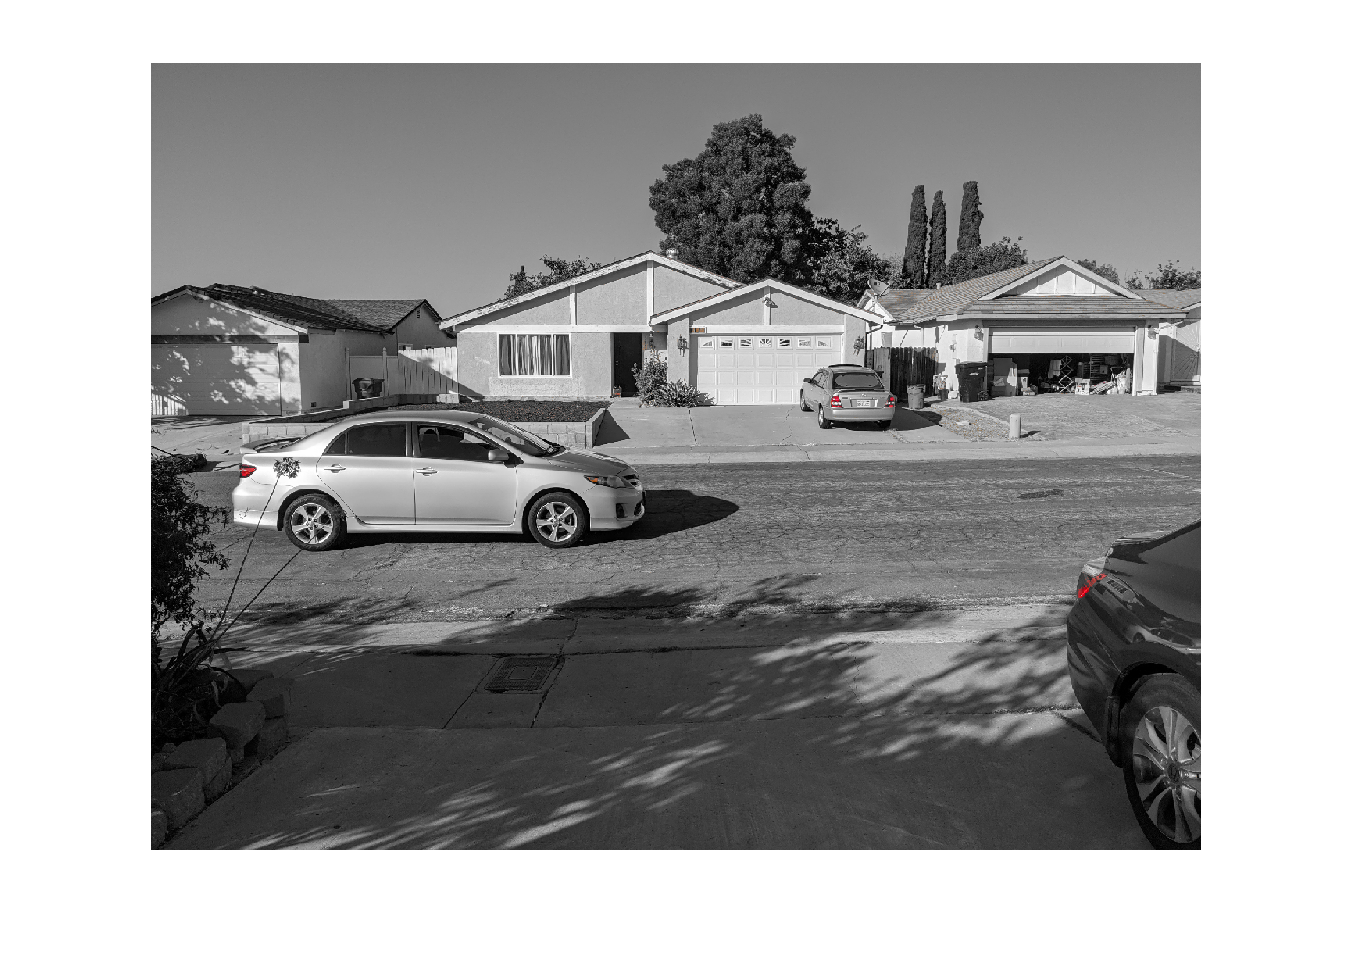
\includegraphics[width = 8.cm]{Images/LeftSingle}
			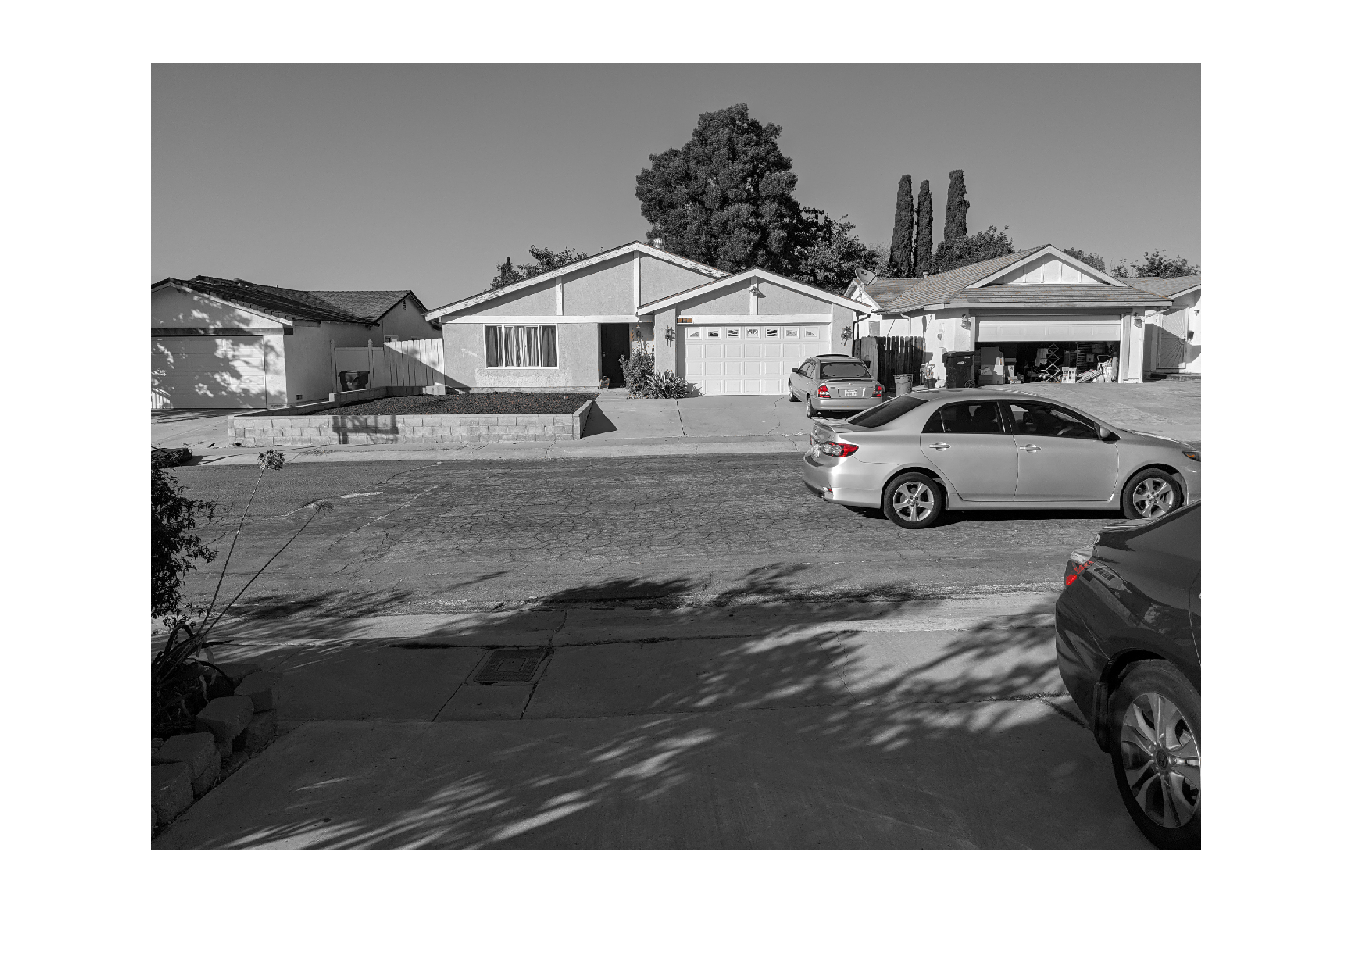
\includegraphics[width = 8.cm]{Images/RightSingle}
		\end{figure}
		\newpage
\begin{lstlisting}[language = Matlab]
a = 0; b = 0; c = 0;

% Point A
for x = (size(imgLeft, 1) / 2) : (2 * size(imgLeft, 1) / 3)
	for y = 1 : (size(imgLeft,2) / 9)
		if (imgLeft(x,y,2) ~= imgLeft(x,y,3))
			a = y;
			break;
		end
	end
	if a ~= 0
		break;
	end
end

% Point B
for x = (size(imgLeft, 1) / 2) : (5 * size(imgLeft, 1) / 8)
	for y = (3 * size(imgLeft, 2) / 8) : (size(imgLeft, 2) / 2)
		if (imgLeft(x,y,2) ~= imgLeft(x,y,3))
			b = y;
			break;
		end
	end
	if b ~= 0
		break;
	end
end

% Point C
for x = (size(imgRight, 1) / 2) : -1 : (size(imgRight, 1) / 3)
	for y = (size(imgRight, 2) / 3) : (2 * size(imgRight, 2) / 3)
		if (imgRight(x,y,2) ~= imgRight(x,y,3))
			c = y;
			break;
		end
	end
	if c ~= 0
		break;
	end
end
\end{lstlisting}
	Results: $a = 353$, $b = 1679$, $c = 2616$.  
	\\ \\
	We get that the distance from Point A to Point B is 1326px.  We get the distance from Point A to Point C is 2263px. Lastly, we get that between each frame is approximately 1.5 seconds.  Now we can solve for speed:
	\[\frac{147\,in}{1326\,px} = \frac{x\,in}{2263\,px} \qquad x = 250.875\,in\]
	\begin{align*}
		\frac{250.875\,in}{1.5\,sec} \cdot \frac{60^2\,sec}{1\,hr} \cdot \frac{1\,mi}{63360\,in} = \frac{9.5\,mi}{hr} 
	\end{align*}
	This is accurate as I was driving between 7 and 10 miles an hour.
	\end{problem}

\end{document}
